\section{Experimental validation}\label{sec:experiments}

In this section, we demonstrate the utility of \ac{CLEAVE} through a series of experiments on an emulated \ac{NCS} running on a number of client devices and a cloudlet.
We aim to answer questions relating to the ability of our framework to provide accurate and repeatable measurements of the performance of \acp{NCS} deployed on edge computing infrastructure.

This section is structured in two parts.
\Cref{ssec:expsetup} details the experimental setup and describes the experiments performed.
\Cref{ssec:results} then presents and discusses the numerical results.

\subsection{Experimental Setup}\label{ssec:expsetup}

We detail our experimental edge setup in \cref{fig:cleave:expsetup,tab:hardware}.
It consists of \num{10} Raspberry Pi 4B  clients connected wirelessly to an IEEE 802.11n \ac{AP}; connected to the Ethernet backbone of this \ac{AP} is a general-purpose Cloudlet.
On top of this physical architecture we configure a Docker Swarm\footnote{Swarm mode overview: \url{https://docs.docker.com/engine/swarm/}} managed centrally from the Cloudlet.
For each experimental scenario we deploy a number of control loops inside this Swarm, executing plant containers exclusively in the Raspberry Pi clients (up to a single plant per client) and controller containers in the Cloudlet.
Plants and controllers communicate using the \ac{UDP} over an overlay network which sits on top of and abstracts away the real network configuration.
Additionally, to obtain baseline results without the stochastic effects of the network, we employ a secondary ``local-only'' setup, in which plants and controllers are executed co-located on the Cloudlet.

% Please add the following required packages to your document preamble:
% \usepackage{booktabs}
% \usepackage{graphicx}
\begin{table}[]
    \centering
    \caption{Hardware used in the experiments.}\label{tab:hardware}
    \resizebox{\columnwidth}{!}{%
    \begin{tabular}{@{}llrrrl@{}}
    \toprule
    \multicolumn{1}{c}{\textbf{}} &
      \multicolumn{1}{c}{\textbf{CPU}} &
      \multicolumn{1}{c}{\textbf{\begin{tabular}[c]{@{}c@{}}Freq\\ {[}\si{\giga\hertz}{]}\end{tabular}}} &
      \multicolumn{1}{c}{\textbf{\begin{tabular}[c]{@{}c@{}}Core\\ Count\end{tabular}}} &
      \multicolumn{1}{c}{\textbf{\begin{tabular}[c]{@{}c@{}}RAM\\ {[}\si{\giga\byte}{]}\end{tabular}}} &
      \multicolumn{1}{c}{\textbf{\begin{tabular}[c]{@{}c@{}}Operating\\ System\end{tabular}}} \\ \midrule
    \textbf{Cloudlet} &
      \begin{tabular}[c]{@{}l@{}}Intel\textregistered{} Core\texttrademark{}\\ i7-8700\end{tabular} &
      \num{3.2} &
      \num{6} &
      \num{32} &
      \begin{tabular}[c]{@{}l@{}}Ubuntu Server \\20.04 LTS \\Kernel v5.4.0\\\ \end{tabular} \\
    \textbf{Client} &
      \begin{tabular}[c]{@{}l@{}}Cortex-A72\\ (ARM v8)\end{tabular} &
      \num{2.0} &
      \num{4} &
      \num{8} &
      \begin{tabular}[c]{@{}l@{}}Ubuntu Server \\20.04 LTS \\Kernel v5.4.0\end{tabular} \\ \bottomrule
    \end{tabular}%
    }
\end{table}

\begin{figure}
    \centering
    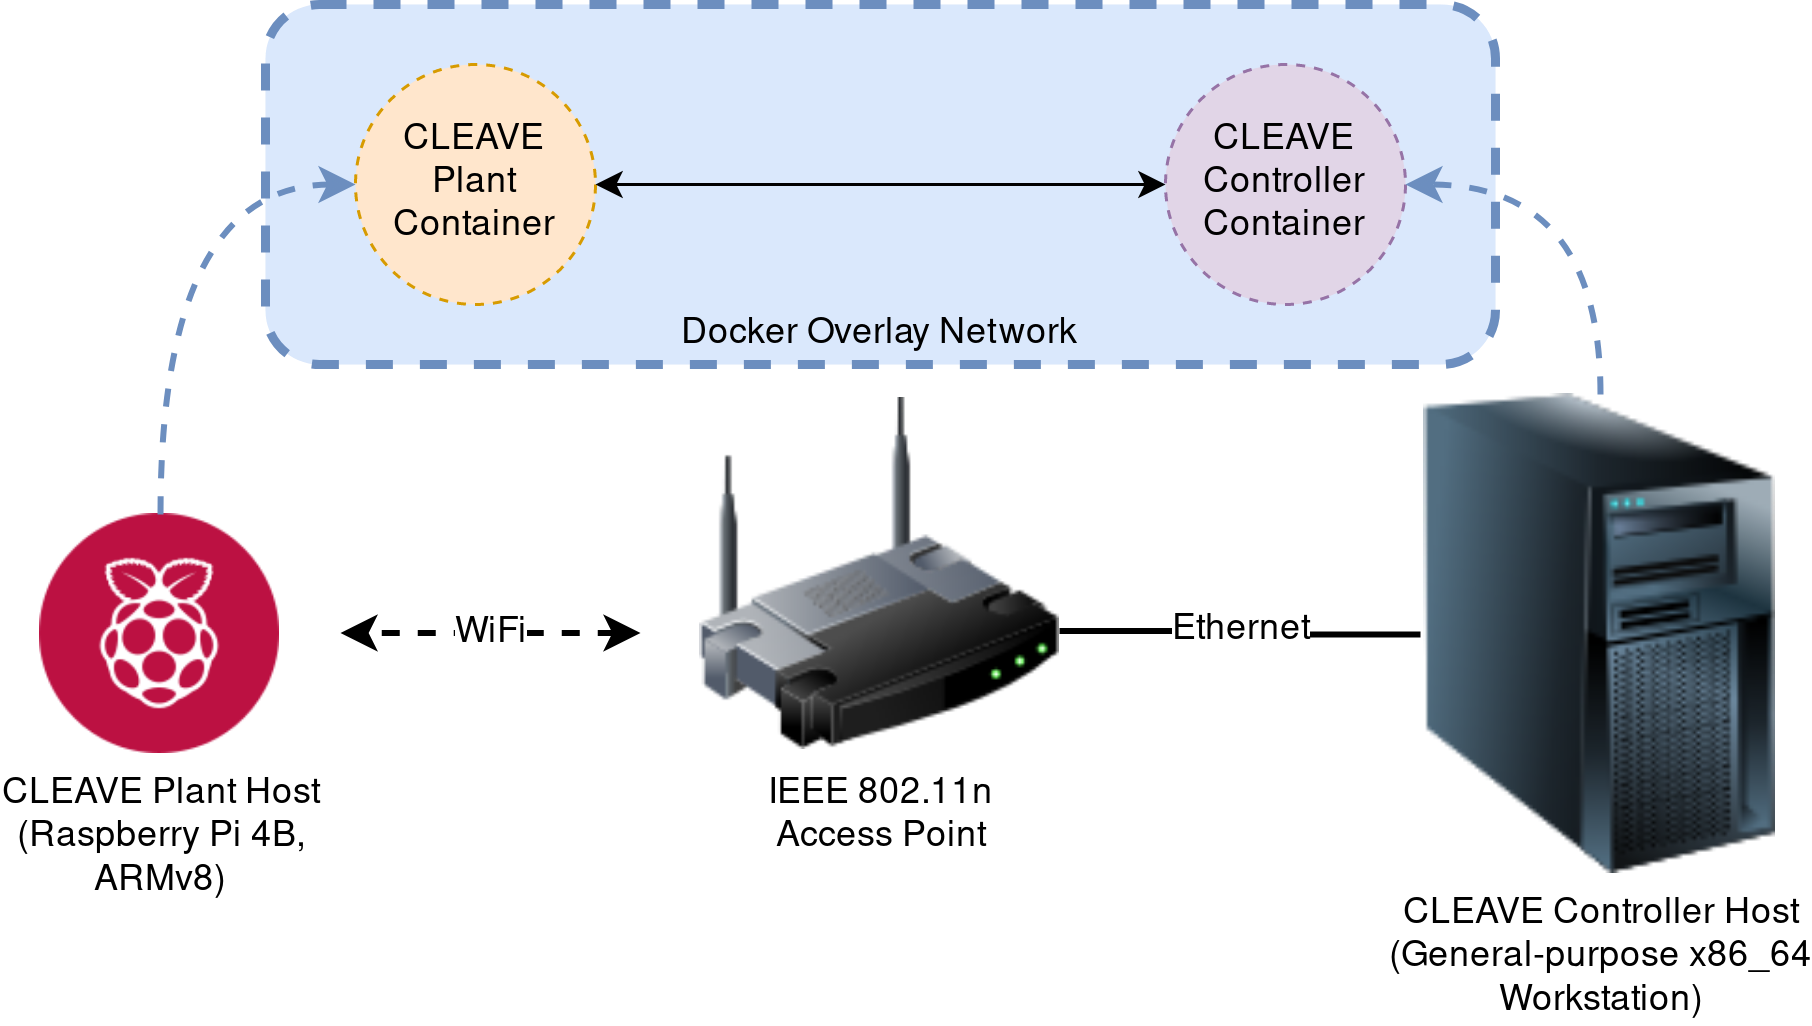
\includegraphics[width=.95\columnwidth]{images/CLEAVE_experiment_setup}
    \caption{
        The setup used for our experimentation. 
        % Containerized versions of the core CLEAVE emulation components are deployed inside a Docker Swarm Overlay Network spanning \num{10} Raspberry Pi 4B clients connected to a single Cloudlet over an IEEE 802.11n \ac{AP}.
    }\label{fig:cleave:expsetup}
\end{figure}

\begin{figure*}[h]
    \centering
    \begin{subfigure}[t]{.5\textwidth}
        \centering
        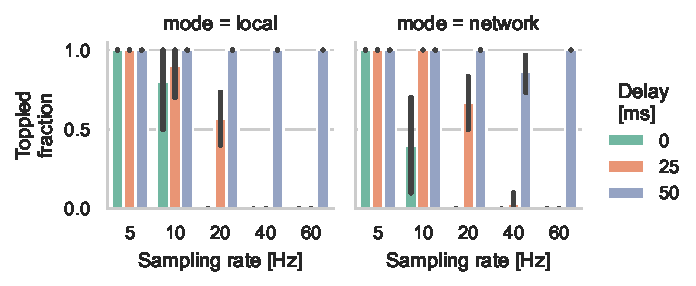
\includegraphics[width=.9\textwidth]{single_loop_toppled}
        \caption{}%
        \label{fig:single:topple}
    \end{subfigure}%
    \begin{subfigure}[t]{.5\textwidth}
        \centering
        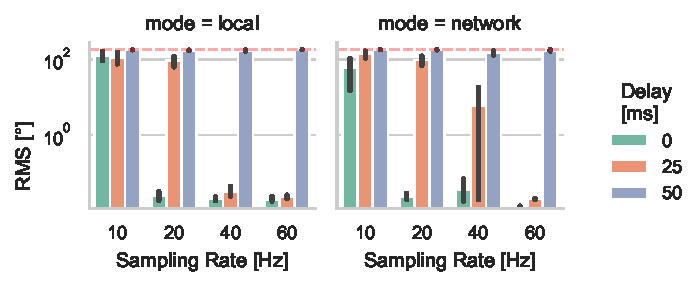
\includegraphics[width=.9\textwidth]{single_loop_rms}
        \caption{}\label{fig:single:rms}
    \end{subfigure}%
    \caption[caption]{
        Stability metrics for the single-loop scenarios.
        \labelcref{fig:single:topple} shows the fraction of plants that toppled, per experimental setup.
        \labelcref{fig:single:rms} shows the \ac{RMS} value of the angle for all pendula that did not topple in the single loop scenarios.
        Error bars indicate \SI{95}{\percent} \acp{CI}.
        }%
    \label{fig:single:stability}
\end{figure*}

\begin{figure}
    \centering
    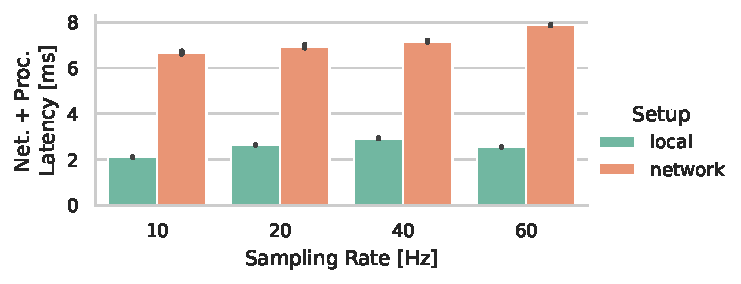
\includegraphics[width=.9\columnwidth]{single_loop_rtts}
    \caption{
        Mean latency due to network and processing for both single-loop scenarios.
        Error bars indicate \SI{95}{\percent} \acp{CI}.
    }\label{fig:single:rtt}
\end{figure}

\begin{figure*}[t]
    \centering
    \begin{subfigure}[h]{.25\textwidth}
        \centering
        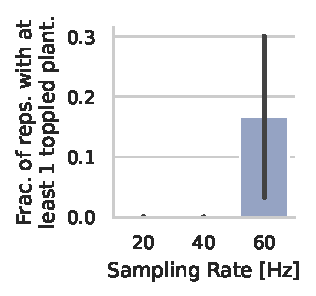
\includegraphics[width=.9\textwidth]{video_topple_frac}
        \caption{}\label{fig:video:toppled}
    \end{subfigure}%
    \begin{subfigure}[h]{.25\textwidth}
        \centering
        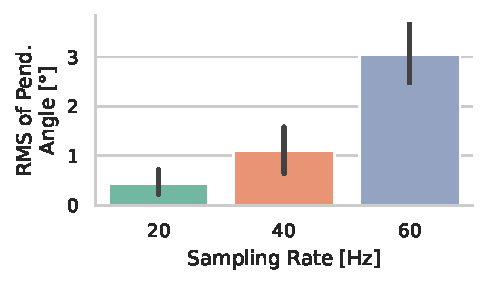
\includegraphics[width=.9\textwidth]{video_angle_rms}
        \caption{}\label{fig:video:rms}
    \end{subfigure}%
    \begin{subfigure}[h]{.25\textwidth}
        \centering
        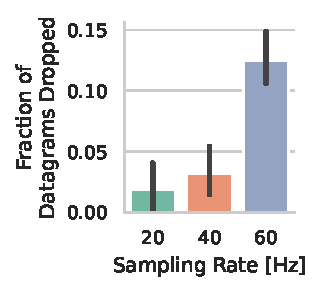
\includegraphics[width=.9\textwidth]{video_drop_frac}
        \caption{}\label{fig:video:drop}
    \end{subfigure}%
    \begin{subfigure}[h]{.25\textwidth}
        \centering
        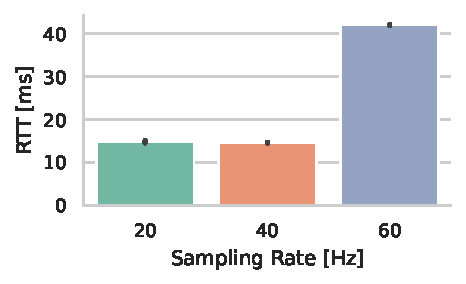
\includegraphics[width=.9\textwidth]{video_rtt}
        \caption{}\label{fig:video:rtt}
    \end{subfigure}%
    \caption{
        Results for the realistic scenario.
        \labelcref{fig:video:toppled} shows the fraction of repetitions of each scenario in which \emph{at least} one plant failed to maintain stability and toppled.
        \labelcref{fig:video:rms} shows the \ac{RMS} for the pendulum angles for each scenario, only considering data from plants that did not topple.
        \labelcref{fig:video:drop} shows the fraction of \ac{UDP} datagrams dropped, averaged over all plants and repetitions per scenario.
        \labelcref{fig:video:rtt} shows the measured end-to-end plant-side \ac{RTT}, averaged over all plants and repetitions per scenario.
        Error bars indicate \SI{95}{\percent} \ac{CI} in all plots.
    }\label{fig:video:results}
\end{figure*}

\subsubsection{Single Loop Baseline Scenarios}

We first run a series of single loop scenarios with varying parametrization of the \ac{NCS}, intended as initial baselines to evaluate the accuracy of the \ac{CLEAVE} framework and showcase its flexibility.

For these scenarios, we vary:
\begin{itemize}
    \item the sampling rate of the Plant state, setting it to \SIlist[list-final-separator={, or }]{10;20;40;60}{\hertz};
    \item the responsiveness of the Controller, adding fixed delays of \SIlist[list-final-separator={, or }]{0;25;50}{\milli\second} after the processing of each sample.
\end{itemize}

We repeat each combination of these parameters at least \num{10} times, for both the networked and ``local-only'' setups; experiments with sampling rates \( \geq \) \SI{20}{\hertz} and artificial delays \( \geq \) \SI{25}{\milli\second} where repeated an additional \num{20} times for better statistical significance.
Each repetition lasts for \SI{5}{\minute}, during which we collect detailed data on both the state of the controlled system as well as on the data sent over the network.

Scenarios are executed automatically in batches using a simple Python script which interacts with Docker through the widely adopted \emph{docker-py}\footnote{Docker SDK for Python: \url{https://docker-py.readthedocs.io/en/stable/}} library.
This is \ac{CLEAVE}'s first advantage over existing frameworks; it is designed with cloud and edge technology and paradigms in mind, making integration with existing systems straightforward.

\subsubsection{Realistic Scenario with Network Resource Contention}

Next, we run a multi-loop scenario to validate the utility of \ac{CLEAVE} in a more realistic setting where network resources are shared with video stream traffic.
Video analytics is one of the main proposed use cases for edge computing~\cite{Ananthanarayanan2017Analytics,Yi2017Analytics,Wang2018Analytics}, and thus we foresee edge \ac{NCS} deployments being deployed in parallel with such applications in the future.

In this scenario, we deploy \num{6} control loops on the experimental setup depicted in \cref{fig:cleave:expsetup}.
On the remaining \num{4} clients we run the \emph{iperf3}\footnote{iperf3: \url{https://iperf.fr/}} traffic load generator, each generating \SI[per-mode=symbol]{6.5}{\mega\bit\per\second} of uplink \ac{UDP} traffic.
This emulates the load generated on the network by \SI{1080}{p} Full-HD video streaming, originating from the clients and terminating in the cloudlet.
We execute this scenario with \ac{NCS} plant sampling rates of \SIlist{20;40;60}{\hertz}.
Each sampling rate configuration is run for \SI{5}{\minute}, and then repeated \num{30} times to obtain statistical significance.
Once again, repetitions of this scenario are executed automatically in batches using a simple Python script and \emph{docker-py}.

\subsection{Results}\label{ssec:results}

The results presented below provide valuable insights on both system limits and on the chosen \ac{NCS} itself, as well as on the capabilities of \ac{CLEAVE}.

\subsubsection{Single Plant Scenario}

We begin with a simple analysis of the stability of the Plant, as \ac{CLEAVE} allows for straightforward and repeatable collection and posterior processing of relevant metrics.  
\cref{fig:single:stability} shows the results relating to the stability of the plants in the single-loop scenarios:
\cref{fig:single:topple} shows the fraction of plants that toppled in each scenario, and \cref{fig:single:rms} shows the average \ac{RMS} for the pendula angles.
Toppled plants were identified simply by analysis of the emulation data; instances whose pendulum angles reached values above a threshold\footnote{This value depends on the parametrization of the controller; in this case it corresponds to \SI{0.35}{\radian}.} were marked as ``toppled''.

As expected, higher sampling rates directly correlate to better quality of control (with the exception of the \SIlist{40;60}{\hertz}, \SI{50}{\milli\second} scenarios --- we attribute this to randomness and the relatively short duration of the experiments).
As sampling rates increased, the system was able to reach stability at higher \acp{RTT}.
These initial results already hint at interesting consequences for \ac{NCS} deployments on the edge.
For instance, it is clear from \cref{fig:single:stability} that network delays can, to a certain extent, be compensated for by increasing the sampling rate of the system.
A corollary of this is that, conversely, at lower network latencies \acp{NCS} are able to stabilize at lower sampling rates.
Adaptive sampling might thus be a straightforward method for optimizing \ac{NCS} resource utilization and energy consumption at the edge.

For completeness, we also showcase \ac{CLEAVE}'s ability to obtain network performance data from the experiments.
\cref{fig:single:rtt} shows average latency due to network and processing (excluding synthetic delays) for both single-loop scenarios.
Packet losses were below \SI{0.2}{\percent} for all parametrizations of the single-loop scenario over the network, and \SI{0}{\percent} for all parametrizations of the local-only setup.

\subsubsection{Realistic Scenario}

In the following, we present and briefly discuss the results for the realistic scenario with network resource contention.

\cref{fig:video:results} shows a summary of the results obtained from the realistic scenario.
These results are interesting in their counter-intuitiveness.
Conventional wisdom would lead us to think that higher sampling rates are always better for the stability of control systems; however, \cref{fig:video:toppled,fig:video:rms} clearly shows this not to be the case for \ac{NCS} in resource-constrained scenarios.
\SI{60}{\hertz} was the least stable configuration, with at least one pendulum toppling in around \SI{16}{\percent} of the repetitions, and average pendulum angle \ac{RMS} about \num{3} times that of the \SI{40}{\hertz} scenario.
\SI{40}{\hertz} was in turn the second worst configuration --- although no pendula toppled in this scenario, average angle \ac{RMS} were double that of the \SI{20}{\hertz} setup.

We can see an explanation for these behaviors in \cref{fig:video:drop,fig:video:rtt}.
Whereas both the \SIlist{20;40}{\hertz} setups show datagram losses well below \SI{5}{\percent}, the \SI{60}{\hertz} scenario shows an average of around \SI{13}{\percent} of datagrams lost.
The differences in \acp{RTT} results are equally dramatic; \acp{RTT} for the \SI{60}{\hertz} scenario were on average approximately \num{3} times those for the \SIlist{20;40}{\hertz} setups (circa \SI{41}{\milli\second} versus \SIrange[range-phrase=--]{13}{15}{\milli\second}).

These results stem from the contention for network resources, and hints at important trade-offs system designers will have to take into consideration when designing and developing \acp{NCS} for deployment on the edge.
The edge will be \emph{multi-tenant} and \emph{multi-instance}. 
\acp{NCS} deployments will have to be designed with shared resources in mind, and given the complexity of these systems, experimental tools like \ac{CLEAVE} will be key for their succesful adoption and massification.
